\subsubsection{Description / circuitry}
% Describe the tractive system active light and additional circuitry. Additionally, fill out the table:

The \gls{tsal} is a distributed system consisting of the following components:
\begin{itemize}
\item Tractive System Active Light mounted on main hoop
\item \gls{tsal} logic \& power circuitry (located in \gls{ecub}; LV only)
\item DC-DC converter to power the \gls{tsal} in case of charged TS but unpowered \gls{glvs} (located in the \gls{acp}; has a \gls{hv} side and a LV side)
\end{itemize}

\paragraph{Tractive System Active Light}

The \gls{tsal} proper is connected with 2 wires. When voltage of 24 V is applied, the \gls{tsal} lights up either in green or red color depending on the polarity.

\begin{figure}[H]
	\centering
	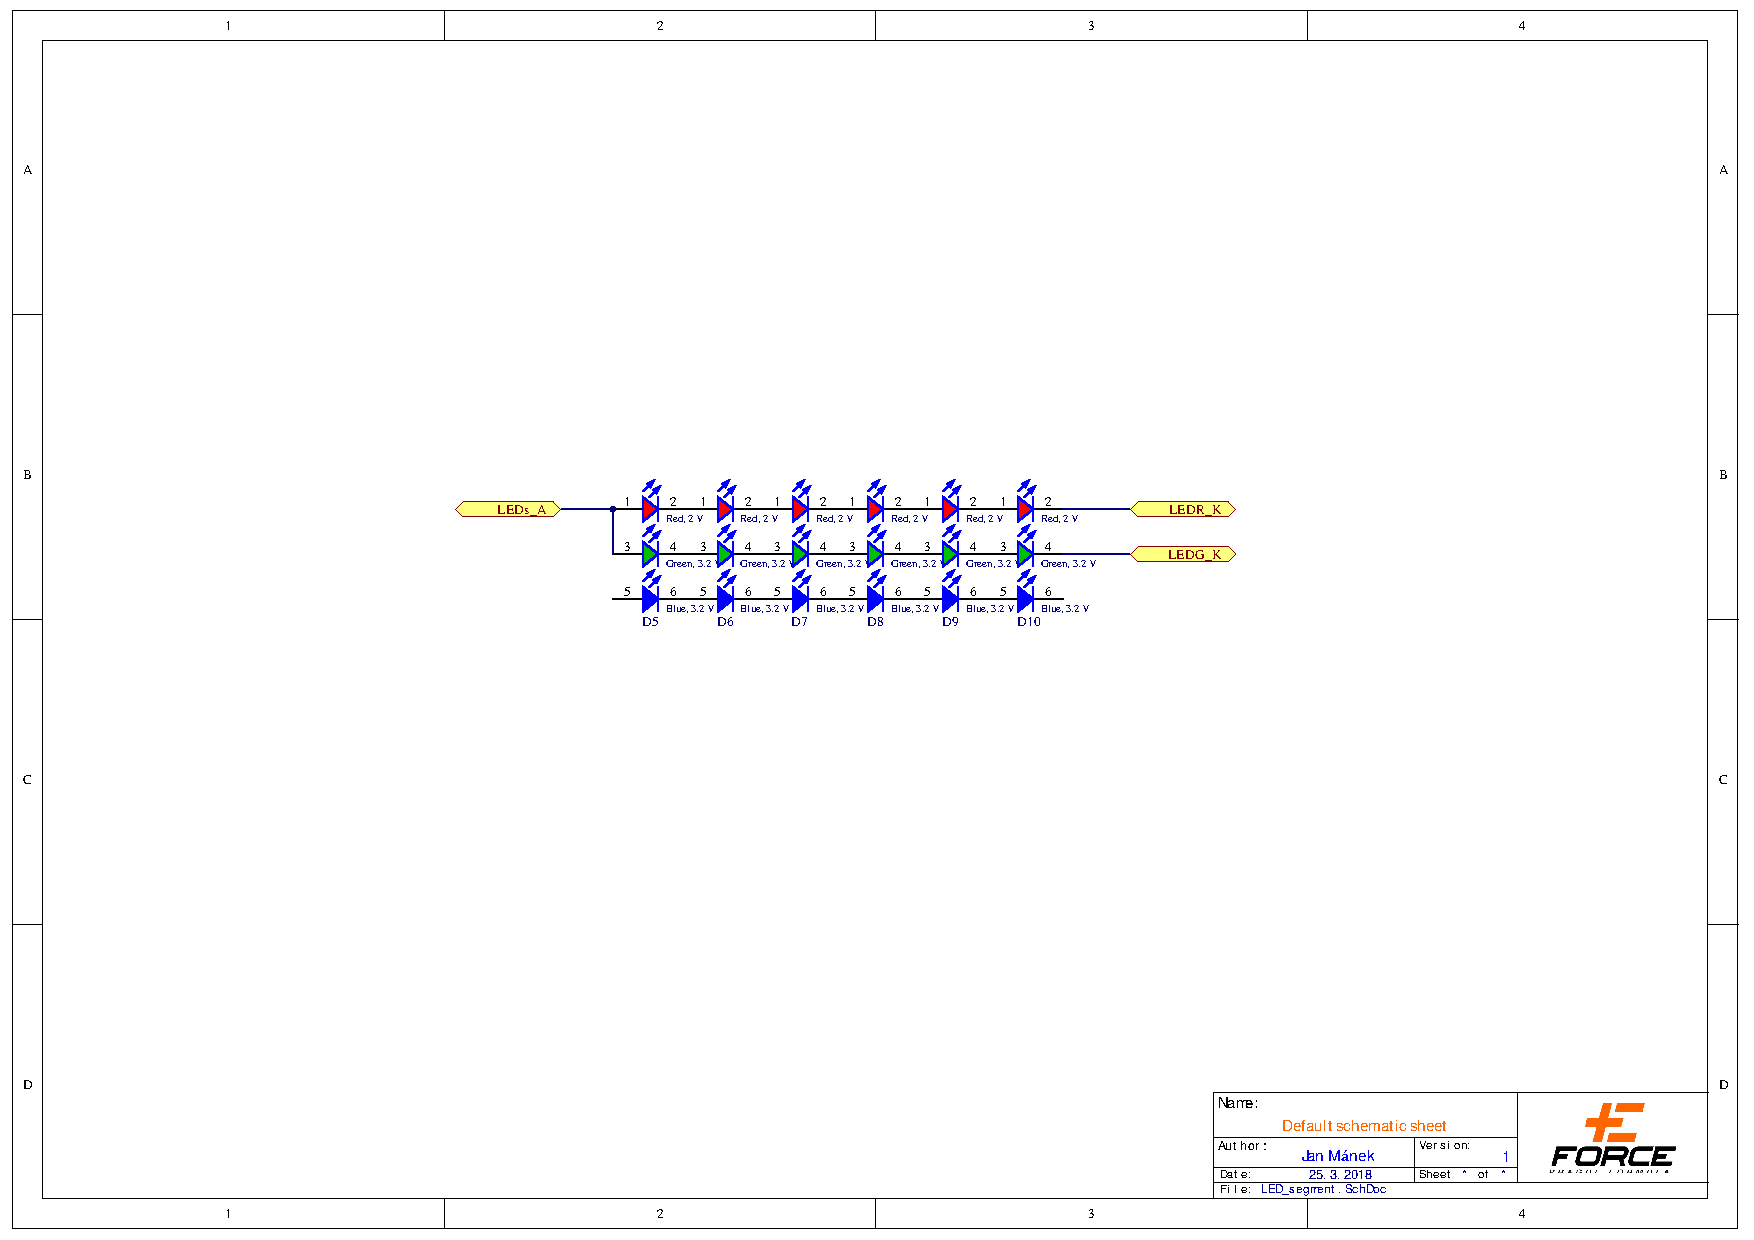
\includegraphics[width=\textwidth,trim={6cm 10cm 6cm 7cm},clip]{./img/TSAL-schematic.pdf}
	\caption{TSAL schematic.}
	\label{fig:TSAL-schematic}
\end{figure}


\begin{table}[H]
	\centering
	\caption{Parameters of the TSAL}
	\begin{tabularx}{\textwidth}{|X|X|}
		\hline
		Supply voltage: & +/- 24VDC \\[\TableSize]
		\hline
		Max. operational current: & 300mA \\[\TableSize]
		\hline
		Lamp type & Bi-color LED \\[\TableSize]
		\hline
		Power consumption: & 7.2 W \\[\TableSize]
		\hline
		Brightness & 124 Lumen (red), 29 Lumen (green) \\[\TableSize]
		\hline
		Frequency: & 3.96Hz \\[\TableSize]
		\hline
		Size (length x height x width): & 128mm x 20mm x 32mm \\[\TableSize]
		\hline
	\end{tabularx}%
	\label{tab:TSAL}%
\end{table}%

\paragraph{TSAL logic \& power circuitry}

To power the \gls{tsal}, a voltage of approximately 24 V is needed. This can be supplied either by the \gls{glvs}, or by a charged Tractive System by means of an isolated DC-DC converter.

A 5V rail is also generated to control all TSAL-related logic. (\ref{fig:TSAL-ECUB-5V})

\begin{figure}[H]
	\centering
	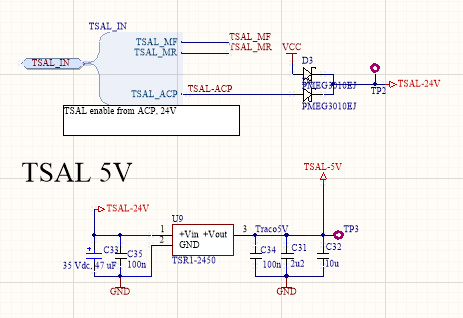
\includegraphics[width=0.6\textwidth]{./img/TSAL-ECUB-5V.png}
	\caption[Powering of the TSAL]{Powering of the \gls{tsal}. \gls{glvs} power is denoted \texttt{VCC}.}
	\label{fig:TSAL-ECUB-5V}
\end{figure}

Discrete logic is used for selecting the light colour. (\ref{fig:TSAL-logic})

\begin{figure}[H]
	\centering
	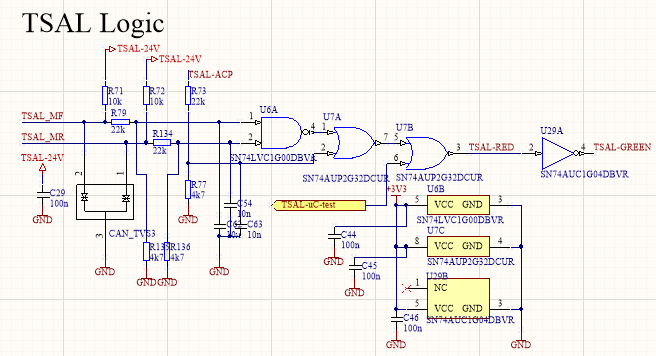
\includegraphics[width=\textwidth]{./img/TSAL-logic.png}
	\caption[TSAL enable logic]{TSAL enable logic. The signals \texttt{TSAL-RED} and \texttt{TSAL-GREEN} are always complementary.}
	\label{fig:TSAL-logic}
\end{figure}

A 555 IC is used to generate the required frequency which is used to modulate the power output. (\ref{fig:TSAL-555})

\begin{figure}[H]
	\centering
	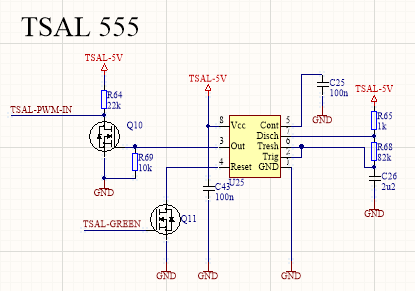
\includegraphics[width=0.6\textwidth]{./img/TSAL-555.png}
	\caption[TSAL frequency generator]{\gls{tsal} frequency generator. When a green light is desired (\gls{glvs} active, \gls{ts} not charged), oscillation is suppressed and the output \texttt{TSAL-PWM-IN} is a constant logical '1'.}
	\label{fig:TSAL-555}
\end{figure}

Finally, a H-bridge is used to drive the proper power outputs with switchable polarity. (\ref{fig:TSAL-H-bridge})

\begin{figure}[H]
	\centering
	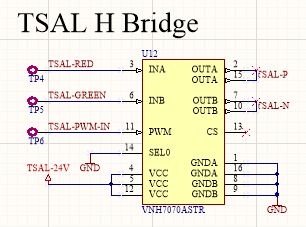
\includegraphics[width=0.5\textwidth]{./img/TSAL-H-bridge.png}
	\caption{\gls{tsal} power H-bridge}
	\label{fig:TSAL-H-bridge}
\end{figure}

\ref{fig:TSAL-logic-table} summarizes operation of the \gls{tsal}.

\begin{table}[H]
	\centering
	\caption{TSAL logic table}
	\begin{tabularx}{\textwidth}{|X|X|X|X|X|}
		\hline
		\textbf{Tractive System state} & \textbf{GLVS state} & \textbf{TSAL powered from} & \textbf{TSAL polarity} & \textbf{TSAL waveform} \\
		\hline
		not charged & off & not powered & -- & -- \\
		\hline
		not charged & on & 24V GLVS & negative (green) & Always-on \\
		\hline
		precharging & on & 24V GLVS & positive (red) & Square wave, 3.96Hz, 50\% duty cycle \\
		\hline
		charged & don't care & TS & positive (red) & Square wave, 3.96Hz, 50\% duty cycle \\
		\hline
	\end{tabularx}%
	\label{fig:TSAL-logic-table}
\end{table}%

\paragraph{DC-DC converter}

To ensure that the \gls{tsal} continues to operate even after disabling \gls{glvs}, the following circuit is used:

\begin{figure}[H]
	\centering
	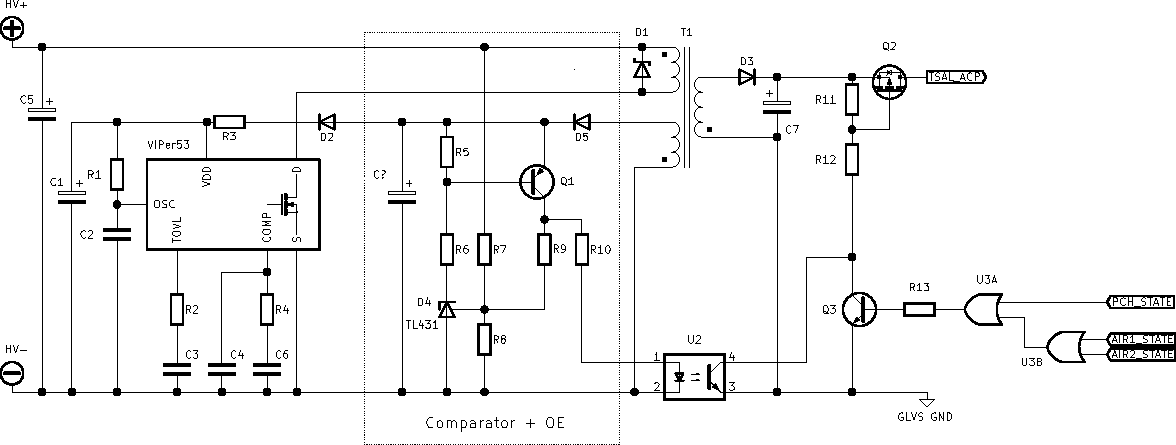
\includegraphics[width=\textwidth]{./img/ECUA_TSAL_POWER.pdf}
	\caption{TSAL HV part schematic.}
	\label{fig:TSAL-HV}
\end{figure}

\paragraph{Explanation of TSAL circuit}
\Gls{tsal} \gls{hv} part schematic \ref{fig:TSAL-HV} is directly connected to the output \gls{hv} pins of \gls{acp}. The circuit is designed with STMicroelectronics chip VIPer53 (\ref{app:viper_datasheet}). The circuit functions as a fly-back DC/DC converter, directly supplying the \gls{tsal}. The converter starts operating at about 40 V, but the output to \gls{tsal} is switched through $Q_2$ only when the HV voltage is more than 60 V. That is ensured using D4, which together with $Q_1$ works as a precise 60 V comparator with a little introduced hysteresis.

The \gls{acp} indication led is powered from the primary side of the transformer, from the VIPER53's own supply voltage.
In case of any of the \glspl{air} closed, or the pre-charge relay contact being detected closed (please see \ref{subsec:precharge}  for details), the \gls{tsal} is supplied from the \gls{glvs} 24 V system, through Q$_2$. The "relay closed" signals from both \glspl{air} and the pre-charge relay are OR-ed together using hardwired logic (i.e. 74LVC2G32).

%schema z backu
\subsubsection{Wiring/cables/connectors}
\iffalse Describe wiring, show schematics, describe connectors and cables used and show useful data regarding the wiring.  Include gauge, voltage and temperature rating of wiring used and any fuses or other overcurrent protection used.\fi

LEDs are supplied from \gls{ecub} (by Harness\_D by connector D1) by 2-wire low voltage cable (\ref{fig:TSAL-wiring}).

\begin{figure}[H]
	\centering
	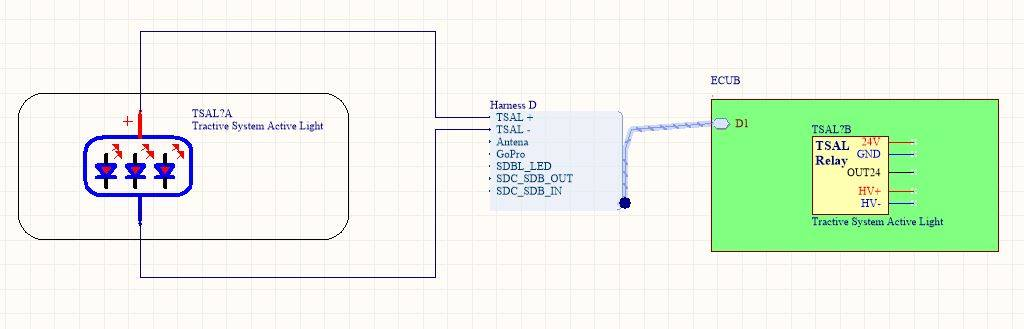
\includegraphics[width=\textwidth,]{./img/tsal-wiring.jpg}
	\caption{Wiring \gls{tsal} from \gls{ecub}}
	\label{fig:TSAL-wiring}
\end{figure}

\subsubsection{Position in car}
%Provide CAD-renderings showing the relevant parts. Mark the parts in the rendering, if necessary.
\gls{tsal} is placed under the main roll hoop, see \ref{fig:TSAL-position}

\begin{figure}[H]
	\centering
	\includegraphics[width=\textwidth,trim={3cm 11cm 2cm 1cm},clip]{./img/tsal-position.pdf}
	\caption{\Gls{tsal} position.}
	\label{fig:TSAL-position}
\end{figure}
